\section{課題2}\label{section:kadai2}
\begin{itembox}{課題2}
  擬似逆行列を計算するプログラムを書き,課題 1 と同じ訓練データから分離超平面を学習せよ.
  また,テストデータの識別率を求めよ.
  クラスラベルについて,$\omega$1 に属するものを 1,$\omega$2 に属するものを-1 などとせよ.さらに,学習された識別面を課題 1 と同じ図に示せ.
\end{itembox}

擬似逆行列を数値計算ライブラリであるnumpyを利用して実装した. 

\begin{eqnarray*}
  A^{+} = (A^{T} \cdot A)^{-1} \cdot A^{T}
\end{eqnarray*}

擬似逆行列を用いて訓練データに関して重みを計算し, 
テストデータによって識別性能を測定したところ,~\ref{section:kadai1} と
同様に0.875という結果だった. 

訓練データ, テストデータおよび識別面を図示したものが
図\ref{fig:kadai2}で, 識別面の位置をウィドロー・ホフのアルゴリズム
によるものと比べてみると, ほぼ同じ位置にあることがわかる. 

\begin{figure}[htbp]
  \centering
  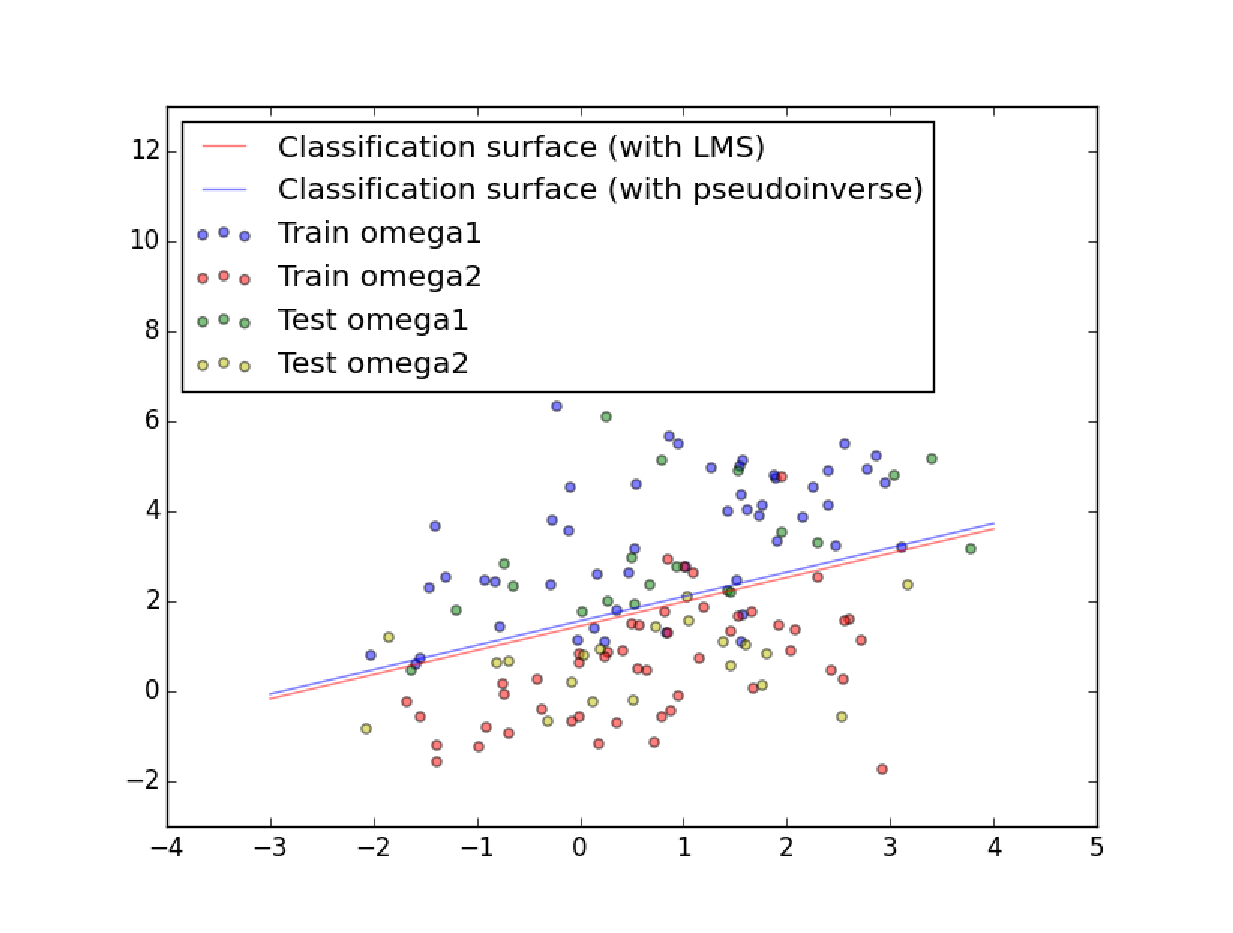
\includegraphics[width=0.8\textwidth]{./assets/kadai2_plot_20150122_031556.eps}
  \caption{データおよび識別面}
  \label{fig:kadai2}
\end{figure}

